\section{A cubic class on weighted compactifications}
\label{sec:compactification}

Lemma~\ref{lem:large-vertex-test} gives vanishing of long products of
projected small diagonals over smooth curve families, modulo the stated
base support.  To apply it on the entire moduli space, we construct a
compact cubic operation whose restriction to a boundary chart differs
from these pure diagonals by controlled terms.  Weighted stable curves
and reduction morphisms are due to Hassett
\cite{Hassett}. The smooth-core configurations below are related to the
blowup compactifications of Fulton--MacPherson \cite{FultonMacPherson}
and their weighted relative versions \cite{Routis}. For rational tails,
Tavakol's proposed comparison with powers of the universal curve
\cite{TavakolRT} was established by Petersen
\cite[Proposition~2.11]{PetersenWonderful}.
Here we also need control under cuts of nodal heavy cores.
The correction at a rational bridge is essential: without it, a codimension-two exceptional class would
remain on a three-light-point configuration space.

We distinguish three cubic objects.  The formal class
$F_J^{\mathrm{st}}$ belongs to the strata algebra and enters the
definition of $Y$.  For the empty heavy set, the corrected weighted
cubic $F^0_{g,\varnothing}$ pulls back under weight reduction to
$q(F_J^{\mathrm{st}})$, with the corresponding label-forgetting pull.
We also use its flagged versions $F^0_{h,B}$, called raw only to
distinguish them from the auxiliary pure lifts $G_{h,B}$.
Each $G_{h,B}$ is obtained from $F^0_{h,B}$ by controlled corrections:
it agrees with the
projected small diagonal over the smooth-core open, not globally
on the compactification.

\subsection{Weighted configurations and cut charts}

Let $(h,B)$ be stable heavy data: $B$ is a finite ordered set and
$2h-2+|B|>0$.  Write
\[
 X_{h,B}(k)=
 \overline{\mathcal M}_{h,(1^B,\epsilon^k)},
 \qquad 0<k\epsilon\leq1,
\]
with $X_{h,B}(0)=\Mbar_{h,B}$.  Here and below any positive rational
weights of total at most one give the same moduli problem for the light
labels.  Lights can coincide with one another, but not with a heavy
marking.  A rational component with one node and only light markings
cannot be stable; a rational component with two nodes and positive light
mass is stable.  These observations also show the independence from the
individual light weights.

The stacks $X_{h,B}(k)$ are smooth and proper, and reduction of weights
and forgetting labels give the usual stabilization morphisms
\cite[Theorem~2.1, Proposition~3.8, Theorems~4.1 and~4.3]{Hassett}.
The one-light space is the universal curve over $\Mbar_{h,B}$:
when its coarse position is a node or a heavy marking, a unique
three-special-point rational component is inserted.  Thus sections and
the relative dualizing line define natural one-light classes.

Fix a stable graph $\Gamma$ of the heavy type.  At its vertex $v$ let
$h_v$ be the genus and let $B_v$ comprise the original heavy markings
and the incident half-edges, all ordered.  Put
\[
 \mathcal B_\Gamma=\prod_v\Mbar_{h_v,B_v},
 \qquad
 \mathcal S_\Gamma=\prod_v\M_{h_v,B_v}.
\]
The \emph{cut chart} with $k$ lights is the disjoint union
\begin{equation}\label{eq:cut-chart}
 X^\Gamma(k)=
 \coprod_{a:\{1,\ldots,k\}\to V(\Gamma)}
 \prod_{v\in V(\Gamma)}X_{h_v,B_v}\bigl(a^{-1}(v)\bigr).
\end{equation}
It has a proper gluing map to the weighted space of the original heavy
type.  Assignments are part of the indexing, so a class supported on
the assignment of specified labels to a vertex means zero on the other
components of \eqref{eq:cut-chart}.

Refining a graph gives further proper cut charts.  These charts cover
the preimage of the corresponding heavy boundary.  Indeed, a node of
the light-forgotten curve may have a chain above it before stabilization.
Choose a node on that chain and cut it, replacing its branches by heavy
flags.  The resulting pieces remain weighted stable; gluing recovers
the original curve.  Several prescribed nodes can be cut independently.
The map on heavy bases is finite, as for the ordinary gluing of stable
curves.

Cutting and light forgetting commute.  The heavy flag replacing a
node branch retains exactly the stability contribution of that branch.
Thus stabilizing on the separate pieces and then gluing gives the same
curve as forgetting and stabilizing after gluing.  This compatibility
will permit operations on unconsumed light labels to pass through any
later cut.

We use rational Chow classes operationally on these smooth stacks.
For an ordinary color space $U$, the arity-indexed operation algebra is
\begin{equation}\label{eq:weighted-operation-algebra}
 \bigoplus_{k\geq0}
 \left(
   \CH^*(X^\Gamma(k))\otimes U^{\otimes k}
                    \otimes\operatorname{sgn}_k
 \right)_{\mathfrak S_k}.
\end{equation}
The product pulls operations to disjoint sets of labels by forgetting
and then multiplies them.  Successive stabilization proves
associativity; exchanging the two sets of labels gives the sign
$(-1)^{k\ell}$.  In particular, cubic and singleton operations are odd
and pair operations are even.  All expressions below are first
identities of labeled classes and then identities in
\eqref{eq:weighted-operation-algebra}.

\subsection{The corrected cubic}

For three light labels define
\begin{equation}\label{eq:weighted-cubic}
 F^0_{h,B}
   =[1=2=3]-\frac12\beta_{h,B}
             +\frac12\sum_{p\in B}\delta_{p,123}\psi_p
       \ \in\CH^2(X_{h,B}(3)).
\end{equation}
The coincidence class is the product of the divisors $[1=2]$ and
$[1=3]$.  The class $\beta_{h,B}$ is defined by taking each stable
one-edge graph of the heavy type, subdividing its edge by a genus-zero
vertex carrying exactly the three lights, and summing the resulting
gluing classes divided by their graph automorphism orders.
The divisor $\delta_{p,123}$ has a tail containing exactly the heavy
mark $p$ and the three lights; $\psi_p$ is the heavy cotangent class on
the weighted space.  Each term in \eqref{eq:weighted-cubic} is symmetric
in the three light labels.

\begin{figure}[tb]
\centering
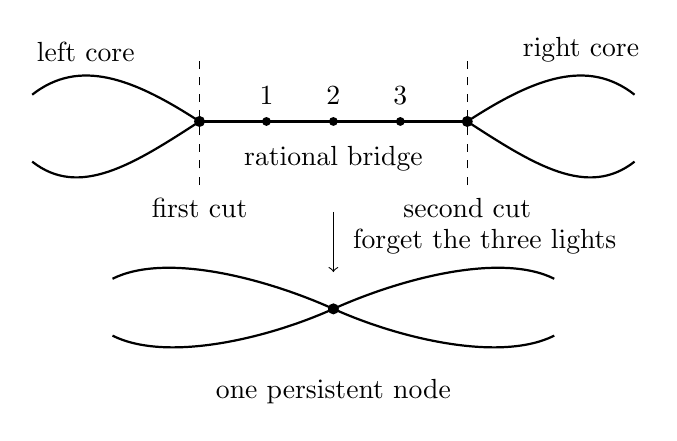
\begin{tikzpicture}[x=.85cm,y=.85cm]
  \draw[thick] (-4.5,.65) .. controls (-3.8,1.2) and (-3,.9) .. (-2,.25);
  \draw[thick] (-4.5,-.35) .. controls (-3.8,-.9) and (-3,-.4) .. (-2,.25);
  \draw[thick] (2,.25) .. controls (3,.9) and (3.8,1.2) .. (4.5,.65);
  \draw[thick] (2,.25) .. controls (3,-.4) and (3.8,-.9) .. (4.5,-.35);
  \draw[thick] (-2,.25) -- (2,.25);
  \fill (-2,.25) circle (2pt);
  \fill (2,.25) circle (2pt);
  \foreach \x/\lab in {-1/1,0/2,1/3}{
    \fill (\x,.25) circle (1.6pt);
    \node[above] at (\x,.36) {$\lab$};
  }
  \draw[dashed] (-2,-.7) -- (-2,1.2);
  \draw[dashed] (2,-.7) -- (2,1.2);
  \node[above] at (-3.7,1.0) {left core};
  \node[above] at (3.7,1.0) {right core};
  \node[below] at (0,.02) {rational bridge};
  \node[below] at (-2,-.75) {first cut};
  \node[below] at (2,-.75) {second cut};
  \draw[->] (0,-1.1) -- (0,-2.0);
  \node[right] at (.15,-1.55) {forget the three lights};
  \draw[thick] (-3.3,-2.1) .. controls (-2.5,-1.7) and (-1,-2.1) .. (0,-2.55);
  \draw[thick] (-3.3,-2.95) .. controls (-2.5,-3.35) and (-1,-3) .. (0,-2.55);
  \draw[thick] (0,-2.55) .. controls (1,-2.1) and (2.5,-1.7) .. (3.3,-2.1);
  \draw[thick] (0,-2.55) .. controls (1,-3) and (2.5,-3.35) .. (3.3,-2.95);
  \fill (0,-2.55) circle (2pt);
  \node[below] at (0,-3.45) {one persistent node};
\end{tikzpicture}
\caption{The two bounding nodes of a light-supported bridge.
After forgetting the lights the bridge contracts.  On a cut chart the
two node conditions contribute two normal cotangent factors.  The same
calculation applies when the two core branches belong to one component.
On the full exceptional surface, coincidence and the bridge class
have integrals $1$ and $2$, respectively, giving
$1-\tfrac12\cdot2=0$.}
\label{fig:bridge-cuts}
\end{figure}



\begin{lemma}\label{lem:weighted-pullback}
Let $g\geq2$, let the heavy set be empty, and pull the three-light
operations to any larger number of light labels by forgetting.
Under weight reduction from ordinary stable pointed curves,
$[i=j]$ pulls back to $\bar D_{ij}$ and $\beta_{g,\varnothing}$
pulls back to the normalized two-edge bridge sum used to define
$\beta_J^{\mathrm{st}}$.
Consequently the coefficient of the prescribed color word in the
signed product of all $F^0_{g,\varnothing}$ pulls back to $q(Y)$,
up to a nonzero rational scalar.
\end{lemma}

\begin{proof}
In codimension one, the inverse image of coincidence consists of
exactly the rational tails containing both labels.  At the generic
point of each tail, the difference of the two coarse positions is a
node-smoothing parameter times a nonzero difference of coordinates on
the tail.  Every multiplicity is therefore one.

Consider next the two bounding nodes of a weighted bridge.  Weight
reduction retaining all labels contracts light-only tails, not a bridge
with positive light mass.  Thus both bounding nodes exist already in
the source, and all the light labels assigned to the bridge originate
between those cuts.  The inverse image is supported on the
corresponding ordinary strata of codimension at least two.  At the
generic two-edge stratum the three labels are distinct on the bridge
and no component is contracted, so the pullback multiplicity is one.
Further collisions add edges and have higher codimension.  Normalized
graph sums count these local cut choices once, including for a loop.
This proves the supported codimension-two pullback assertion.

Forgetting commutes with reduction.  Finally, extracting a fixed color
word from signed averaging retains exactly the permutations preserving
that word, with their signs.  Depending on the averaging convention
there is a positive factorial denominator, but no zero scalar.
\end{proof}

\subsection{The local three-position calculation}

Over $\mathcal S_\Gamma$ let $C_v$ denote the smooth core curve at
vertex $v$.  For a fixed assignment of three labels, there is a coarse
position map
\begin{equation}\label{eq:coarse-positions}
 c:X^\Gamma(3)|_{\mathcal S_\Gamma}
       \longrightarrow
       C_{a(1)}\times_{\mathcal S_\Gamma}
       C_{a(2)}\times_{\mathcal S_\Gamma} C_{a(3)}.
\end{equation}
All products in this subsection are over the indicated heavy base.

\begin{lemma}\label{lem:three-position-blowup}
The map \eqref{eq:coarse-positions} is the iterated blowup obtained,
at each flag $p$, by first blowing up the locus where all three
assigned positions equal $p$, when present, and then the strict
transforms of the loci where two assigned positions equal $p$.
The latter centers are disjoint after the first blowup.
\end{lemma}

\begin{proof}
Extra components above a smooth pointed core are chains attached at
its flags.  A branch with no heavy endpoint and only light markings
would have a terminal light-only tail and is impossible.  Every level
of a chain carries positive light mass.

Choose a local parameter at a flag and write $x_i$ for the corresponding
coarse coordinate of label $i$.  The zero divisor of $x_i$ on the
configuration space is the sum, with multiplicity one, of the cuts
moving that label onto the expanded chain.  The multiplicity follows
from a one-node smoothing $xy=t$.  At a fixed point of the
configuration space these cuts form an initial segment of the
ordered chain.  Hence the products of smoothing parameters occurring
in the different $x_i$ are ordered by divisibility.  In particular,
each relevant pair or triple ideal is principal after pullback.
This gives a morphism to the first blowup and then to the successive
pair blowups; after the first step the pulled pair ideal is its strict
transform ideal times the exceptional line.

The blowup ratios recover the expanded configuration.  On a level
put its outward endpoint at infinity and its inward endpoint at zero.
The leading ratios of coarse coordinate differences are the ratios
of the light coordinates on that level, modulo common scaling.
Labels on separate levels give the limiting ratios zero or infinity.
Forgetting to pairs gives all these ratios compatibly, so the ratios
determine the levels and their configurations.  Automorphisms fixing
the core and the marked lights are trivial.  The resulting
representable map to the iterated blowup is therefore quasi-finite.
It is also proper and birational.  The target is smooth, and the
source is smooth by weighted deformation theory; working on
an etale chart of the core data, a proper birational quasi-finite map
to this normal target is an isomorphism
\cite[Tags~02LS and~0AB1]{Stacks}.

In the first exceptional plane, the strict pair centers meet at the
three distinct coordinate points, proving their disjointness.
The constructions at distinct flags have disjoint centers.
\end{proof}

Denote the total first exceptional divisor at a triple flag locus by
$E_{p,123}$.  Denote pair exceptional divisors, preferably pulled back
from the corresponding two-light spaces, by $E_{p,ij}$.
The blowup formula for Chow groups \cite[Proposition~6.7(e)]{Fulton} shows that a
codimension-two class on \eqref{eq:coarse-positions} has, in addition to
its main pullback, terms of the following forms:
\begin{equation}\label{eq:blowup-components}
 E_{p,ij}\,A_{p,ij},\qquad
 E_{p,123}\,D_p,\qquad
 a_p E_{p,123}^{\,2}.
\end{equation}
Here $A_{p,ij}$ is a divisor class on the remaining curve over the
base, $D_p$ is a base divisor class, and $a_p$ is a scalar on each
connected component of the base.  For clarity, if \(E_{p,ij}^{\mathrm{str}}\) is the strict pair
exceptional divisor and \(E_{p,ij}^{\mathrm{pull}}\) is pulled back
from two labels, then
\[
 E_{p,ij}^{\mathrm{pull}}
   =E_{p,ij}^{\mathrm{str}}+E_{p,123}.
\]
Multiplying the difference by a divisor on the remaining curve
restricts that divisor, on \(E_{p,123}\), to the flag section.
It is therefore a pulled base divisor. Replacing the strict version
by the pulled version changes only the
triple-exceptional-times-base-divisor term, and introduces no new
scalar multiple of \(E_{p,123}^2\).  Formula
\eqref{eq:blowup-components} includes assignments to different
vertices, in which some of the centers are simply absent.

When a raw class $F^0$ is pulled from an ancestor chart, its main
component is the small diagonal if all three labels are assigned to
one relevant descendant vertex, and is zero otherwise.  Away from
flags this is immediate.  The coincidence, bridge, and heavy-tail
corrections not seen there project to loci where all three coarse
positions are flags, of codimension three; they cannot alter a main
codimension-two class.

For the same pulled raw class, the divisor coefficients $A_{p,ij}$ in
\eqref{eq:blowup-components} are supported on flag sections of the
remaining curve, up to base divisor terms.  To see this, remove all
flags from that remaining curve.  Neither the raw class nor its main
diagonal pullback meets the pair exceptional locus over this open.
Intersecting with the exceptional divisor and pushing to its center
recovers its coefficient, with the usual negative self-intersection
sign for a codimension-two blowup center.  The coefficient is
therefore zero on this open.  Chow localization on the curve over the
base gives the assertion.

\begin{lemma}\label{lem:triple-exceptional-cancellation}
For the pullback of a raw cubic class $F^0$ from an ancestor chart, the
coefficient $a_p$ in \eqref{eq:blowup-components} is zero at every
triple flag locus.
\end{lemma}

\begin{proof}
Work first over a field point of the smooth heavy base.  The full
fiber over three positions at one flag is the weighted chain space
with two heavy endpoints and three lights, the Losev--Manin surface
\cite[Theorems~2.2 and~2.6.3]{LosevManin},
\cite[\S6.4]{Hassett}. By
Lemma~\ref{lem:three-position-blowup}, it is the first exceptional
$\mathbb P^2$ blown up at its three pair-collision points.
The total class $E_{p,123}$ restricts to the pullback of
$\mathcal O_{\mathbb P^2}(-1)$; hence
\begin{equation}\label{eq:exceptional-square}
 \int E_{p,123}^{\,2}=1.
\end{equation}
Main pullbacks, pair terms multiplied by a remaining-position divisor,
and base terms have integral zero on this fiber.  Thus this integral
detects exactly $a_p$.

The coincidence term gives one: its locus is the single transverse
configuration in which the three lights coincide away from the
endpoints.  We distinguish new and inherited flags relative to the
ancestor supplying the raw cubic.  Suppose first that $p$ is a new cut
flag.  There is one pair of bounding nodes isolating the chain carrying
the three lights.
This remains true on the boundary of the chain space.  Indeed, a
subcurve contracted upon forgetting the lights has two endpoint flags
and no persistent heavy marking; every component has at least two
incident branches before counting lights, so the component tree must
be a chain, with positive light mass on every level.  Its extreme
bounding nodes are uniquely determined.

With these cuts distinguished, as in Figure~\ref{fig:bridge-cuts},
the bridge locus is a regular
two-node condition in a versal deformation chart.  Its two normal
lines are the tensor products of the corresponding branch tangent
lines.  The core factors are constant on our fiber, so its
self-intersection restricts to
\begin{equation}\label{eq:bridge-normal}
 (-\psi_0)(-\psi_\infty)=\psi_0\psi_\infty.
\end{equation}
The normalized bridge sum counts this local branch once.  This
argument also treats a self-node: one distinguishes the two branches
before applying the normal formula, and the graph automorphism factor
removes the duplicate ordering.

Reduction from $\Mbar_{0,5}$ to the chain space preserves both heavy
cotangent lines.  A rational component carrying a heavy mark cannot
be contracted when the other three weights are decreased but remain
positive.  The genus-zero string recurrence gives
\begin{equation}\label{eq:chain-cotangent-integral}
 \int_{\Mbar_{0,5}}\psi_0\psi_\infty
   =\int_{\Mbar_{0,4}}\psi_0
     +\int_{\Mbar_{0,4}}\psi_\infty
   =2.
\end{equation}
The last equality follows by forgetting once more to
$\Mbar_{0,3}$.  Equivalently,
\eqref{eq:chain-cotangent-integral} is the degree-two case of the
genus-zero cotangent integral formula.  The bridge contribution to
$F^0$ is therefore $-\tfrac12\cdot2=-1$, canceling coincidence.

If instead $p$ is an inherited heavy flag, the relevant term is the
unique outer tail with that heavy marking and all three lights.
Its normal factor is $-\psi_0$ on the chain and the inserted
$\psi_p$ is $\psi_\infty$.  Thus
$\delta_{p,123}\psi_p$ has integral $-2$, and its coefficient
$+\tfrac12$ again cancels coincidence.  No other bridge or heavy-tail
type meets this fiber: after the lights are forgotten its contracted
locus is this specified node or this specified heavy mark.

We have shown that the scalar coefficient in
\eqref{eq:blowup-components} is zero on every connected smooth-core
base component.  This proves the result over that base.
\end{proof}

\subsection{Controlled pure lifts}

For a smooth heavy core $\pi:C\to S$, choose a degree-one rational
class
\[
 e_C=
 \begin{cases}
 [p],&\text{if a heavy flag $p$ has been chosen},\\
 c_1(\omega_{C/S})/(2h-2),&\text{if $B=\varnothing$}.
 \end{cases}
\]
The second case occurs only for $h\geq2$.  As in the curve tensor
construction, put
\begin{equation}\label{eq:compact-centering}
 e_C'=e_C-\frac12\pi^*\pi_*(e_C^2),
 \qquad
 \eta_C=[\Delta_C]-e'_{C,1}-e'_{C,2}.
\end{equation}
Write $\Delta_C^{\mathrm{pure}}$ for the small diagonal projected by
$\eta_C$ in each of its three slots.  Expanding the three projectors
shows that
\begin{equation}\label{eq:nonpure-pair-singleton}
 \begin{gathered}
 [\Delta_{123}]-\Delta_C^{\mathrm{pure}}
 \quad\text{is a sum of pair--singleton products},\\
 \text{with singleton factors }1_C\text{ or }e_C'.
 \end{gathered}
\end{equation}
No numerical equivalence is used in this expansion: it is the
decomposition of the diagonal correspondence into the pure projector
and the two hyperbolic projectors.

\begin{proposition}[Controlled pure lifts]
\label{prop:controlled-lifts}
For every stable heavy type $(h,B)$ one can choose a symmetric class
$G_{h,B}\in\CH^2(X_{h,B}(3))$ with the following properties.
\begin{enumerate}[label=\textup{(\roman*)}]
\item
Over the smooth heavy base, $G_{h,B}$ is exactly the pullback of
$\Delta_C^{\mathrm{pure}}$ by the coarse-position map.
\item
Pull a raw cubic $F^0$, or one of these chosen pure lifts $G$, from any
ancestor chart to a compact descendant cut chart.  Its operation is
a sum of the chosen pure lifts at the relevant descendant vertices,
with all three labels assigned to that vertex, together with
pair-times-singleton operations and a residual cubic operation.
\item
The singleton operations in \textup{(ii)}, and all their further
pullbacks through cuts and light forgetting, are controlled as
follows.  Over fixed smooth core data their restrictions lie
componentwise in the span of the unit, the canonical class, and the
flag points.  On any smooth test family the same statement holds
modulo classes supported over positive base codimension.
\item
On the current smooth-core open the residual operation in
\textup{(ii)} is a finite sum of classes containing a pulled base
divisor factor.  The base divisor may come from the current heavy
base or from a compact ancestor base.  Consequently its pullback to
every smooth test family is zero operationally after removing a
positive-codimension subset of that test base.
\end{enumerate}
All expansions preserve the color multiset.  They may always use one
and the same chosen $G$ and centering at a given current vertex,
regardless of which ancestor supplied the operation.
\end{proposition}

\begin{proof}
First work on the smooth heavy base of the class itself.  The blowup
decomposition \eqref{eq:blowup-components} and
Lemma~\ref{lem:triple-exceptional-cancellation} express $F^0$ as the
pullback of the small diagonal, plus pair-exceptional-times-singleton
terms and triple-exceptional-times-base-divisor terms.  Subtract these
terms, and also subtract \eqref{eq:nonpure-pair-singleton}.

These subtractions have compact extensions with the required
structure.  A pair exceptional divisor extends as the heavy-flag
tail boundary on the two-light space; a triple exceptional divisor
extends as its three-light counterpart.  Divisor coefficients on
the heavy base extend by Chow localization.  Pair coefficients may
also be extended by Chow localization on the smooth compact
two-light stack.  The singleton factors have specific extensions:
use units, the heavy sections, the relative dualizing line on the
one-light universal curve, and base classes.  In particular we do
not choose an arbitrary compact extension of the pure diagonal.
Define $G$ by making these structured subtractions from $F^0$, and
average over the three labels.  This gives \textup{(i)}.

Now pull to a deeper cut chart.  The raw $F^0$ has the decomposition
just proved there.  Its main component is the sum of the small
diagonals of the relevant descendant vertices.  Replace each by the
corresponding chosen $G$ plus its structured corrections.
Inherited pair-times-singleton subtractions retain that form:
forgetting commutes with cutting, so the pair coefficient remains a
two-label operation and the singleton remains a one-label operation.
The former is allowed to be arbitrary.  For the latter, the
normalization formula for the dualizing line gives the canonical
class plus the new branch points on each component.  A section
either lies on the relevant component or has zero restriction there;
base terms remain base terms.  This proves the asserted span and its
stability under further cuts.

The only other corrections are exceptional divisors multiplied by
base divisor classes.  On pulling an inherited correction, the
exceptional factor need not have a special form, but its base
divisor factor remains pulled from the ancestor heavy base.
The same description applies to the new corrections on the current
chart.  Thus the residual over its smooth-core open is of the form
\begin{equation}\label{eq:controlled-residual}
 \sum_j H_j\cdot\rho_j^*D_j,
\end{equation}
where $H_j$ is a one-codimensional three-label operation and $D_j$
is a divisor class on a current or ancestor heavy base, with the
natural induced map $\rho_j$.
Extending this decomposition to the compact chart can also leave a
difference supported over its heavy boundary, by Chow localization.
Include that difference in the residual operation.  Its restriction to
the smooth-core open is zero, so the residual there still has precisely
the form \eqref{eq:controlled-residual}.

To verify the last assertion after an arbitrary smooth test base
change $S$, represent each pulled rational divisor class by the
first Chern class of a rational line bundle.  A rational
trivialization makes it zero off a divisor of $S$.  After removing
the finite union of these divisors, every summand of
\eqref{eq:controlled-residual} is zero as an operational class.
This remains true if the image of $S$ lies inside a divisor on an
ancestor base: it is the pulled line bundle on $S$, not a presumed
transverse pullback of its original supporting cycle, that is used.
The base corrections in $e_C'$ are covered by the same argument.

Finally, if a previous operation used a different centering or a
different inherited presentation, expand it through its raw $F^0$
and the structured subtractions defining that presentation.  The
preceding argument again leaves the same allowed pair and singleton
terms, and a residual of the stated form on the smooth-core open.
We may therefore re-expand to
the fixed choice of $G$ at every current vertex.  Assignment
conditions can be imposed separately on the pair and singleton
factors by making their operations zero on the other components of
the disjoint union \eqref{eq:cut-chart}.  All steps occur before
inserting colors, and so preserve their multiset.
\end{proof}

\begin{remark}\label{rem:family-not-fiber}
The conclusion in Proposition~\ref{prop:controlled-lifts}\textup{(iv)}
is stronger than vanishing on individual geometric fibers.  It gives
operational vanishing on an open of every smooth test family,
including families mapping into a special locus of the heavy base.
This is the form needed when the remaining operation is multiplied
by an arbitrary cycle and Chow localization is used to lower its
base support.  Likewise, on the smooth-core open the equality in
\textup{(i)} is an equality of relative Chow correspondences.
Smooth proper base change for their pull, intersection, and push
operations identifies it with the centered tensor construction on
any such test family.
\end{remark}
